\documentclass[12pt]{article}
\usepackage[spanish]{babel}
\usepackage[utf8]{inputenc}
\usepackage{amsmath}
\usepackage{graphicx}
\usepackage{booktabs}
\usepackage{array}
\usepackage{multirow}
\usepackage{float}
\usepackage{longtable}
\usepackage{subcaption}
\usepackage{wrapfig}
\usepackage{tikz}
\usetikzlibrary{arrows.meta, positioning, shapes.geometric}
\title{Proyecto 3: Reemplazo de Equipos}
\author{Emily Sanchez \\ Viviana Vargas \\[1cm] Curso: Investigación de Operaciones \\ II Semestre 2025}
\date{\today}

\begin{document}

\maketitle
\newpage
\section*{Problema de Reemplazo de Equipos}
El problema consiste en determinar el momento óptimo para reemplazar un equipo durante un período de planificación.\\
\textbf{Fórmula del costo:} $C_{t,j} = \text{Compra} + \sum_{k=1}^{j-t} \text{Mantenimiento}_k - \text{Venta}_{j-t}$\\
\textbf{Algoritmo:} Programación Dinámica hacia atrás\\
\textbf{Función recursiva:} $g(t) = \min\limits_{j=t+1}^{\min(t+\text{vida útil}, n)} \{C_{t,j} + g(j)\}$ con $g(n) = 0$\\

\section*{Datos del Problema}
\begin{itemize}
\item Costo inicial (compra): \$650,00
\item Plazo del proyecto: 6 años
\item Vida útil del equipo: 4 años
\end{itemize}

\begin{table}[H]
\centering
\caption{Datos del equipo por año de uso}
\begin{tabular}{ccc}
\toprule
Año de Uso & Mantenimiento & Valor Residual \\
\midrule
1 & \$50,00 & \$550,00 \\
2 & \$65,00 & \$450,00 \\
3 & \$75,00 & \$350,00 \\
4 & \$95,00 & \$250,00 \\
\bottomrule
\end{tabular}
\end{table}

\clearpage
\section*{Cálculo de Costos $C_{t,j}$}
\begin{longtable}{cccc}
\caption{Cálculo detallado de costos por período} \\
\toprule
Período (t-j) & Duración & Fórmula & Costo \\
\midrule
\endfirsthead
\toprule
Período (t-j) & Duración & Fórmula & Costo \\
\midrule
\endhead
\bottomrule
\endfoot
\bottomrule
\endlastfoot
0-1 & 1 año & $650 + 50 - 550$ & \$150,00 \\
0-2 & 2 años & $650 + 50 + 65 - 450$ & \$315,00 \\
0-3 & 3 años & $650 + 50 + 65 + 75 - 350$ & \$490,00 \\
0-4 & 4 años & $650 + 50 + 65 + 75 + 95 - 250$ & \$685,00 \\
1-2 & 1 año & $650 + 50 - 550$ & \$150,00 \\
1-3 & 2 años & $650 + 50 + 65 - 450$ & \$315,00 \\
1-4 & 3 años & $650 + 50 + 65 + 75 - 350$ & \$490,00 \\
1-5 & 4 años & $650 + 50 + 65 + 75 + 95 - 250$ & \$685,00 \\
2-3 & 1 año & $650 + 50 - 550$ & \$150,00 \\
2-4 & 2 años & $650 + 50 + 65 - 450$ & \$315,00 \\
2-5 & 3 años & $650 + 50 + 65 + 75 - 350$ & \$490,00 \\
2-6 & 4 años & $650 + 50 + 65 + 75 + 95 - 250$ & \$685,00 \\
3-4 & 1 año & $650 + 50 - 550$ & \$150,00 \\
3-5 & 2 años & $650 + 50 + 65 - 450$ & \$315,00 \\
3-6 & 3 años & $650 + 50 + 65 + 75 - 350$ & \$490,00 \\
4-5 & 1 año & $650 + 50 - 550$ & \$150,00 \\
4-6 & 2 años & $650 + 50 + 65 - 450$ & \$315,00 \\
5-6 & 1 año & $650 + 50 - 550$ & \$150,00 \\
\bottomrule
\end{longtable}

\clearpage
\section*{Cálculo de $g(t)$ (Programación Dinámica)}
\begin{itemize}
\item $g(6) = 0$ (caso base)
\item $g(5) = \min\{ C_{5,6} + g(6) = 150,00\} = \$150,00$
\item $g(4) = \min\{ C_{4,5} + g(5) = 300,00, C_{4,6} + g(6) = 315,00\} = \$300,00$
\item $g(3) = \min\{ C_{3,4} + g(4) = 450,00, C_{3,5} + g(5) = 465,00, C_{3,6} + g(6) = 490,00\} = \$450,00$
\item $g(2) = \min\{ C_{2,3} + g(3) = 600,00, C_{2,4} + g(4) = 615,00, C_{2,5} + g(5) = 640,00, C_{2,6} + g(6) = 685,00\} = \$600,00$
\item $g(1) = \min\{ C_{1,2} + g(2) = 750,00, C_{1,3} + g(3) = 765,00, C_{1,4} + g(4) = 790,00, C_{1,5} + g(5) = 835,00\} = \$750,00$
\item $g(0) = \min\{ C_{0,1} + g(1) = 900,00, C_{0,2} + g(2) = 915,00, C_{0,3} + g(3) = 940,00, C_{0,4} + g(4) = 985,00\} = \$900,00$
\end{itemize}

\clearpage
\section*{Solución Óptima}
\textbf{Costo mínimo total:} \$900,00\\
\textbf{Planes óptimos encontrados:} 1
\subsection*{Grafos de Planes Óptimos}
A continuación se presentan los grafos de \emph{saltos de rana} para cada plan óptimo encontrado.

\begin{figure}[H]
\centering
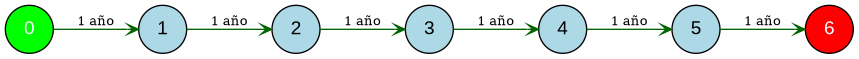
\includegraphics[width=0.8\textwidth]{1111_plan_1.png}
\caption{Plan Óptimo 1: \texttt{0-1-2-3-4-5-6}}
\label{fig:plan1}
\end{figure}

\textbf{Plan 1:} \texttt{0-1-2-3-4-5-6}
\begin{itemize}\small
\item Período 0-1: 1 año, Costo: \$150,00
\item Período 1-2: 1 año, Costo: \$150,00
\item Período 2-3: 1 año, Costo: \$150,00
\item Período 3-4: 1 año, Costo: \$150,00
\item Período 4-5: 1 año, Costo: \$150,00
\item Período 5-6: 1 año, Costo: \$150,00
\end{itemize}

\subsection*{Resumen de Planes}
\begin{itemize}
\item \textbf{Plan 1:} 0-1-2-3-4-5-6
\end{itemize}
\begin{table}[H]
\centering
\caption{Resumen de costos mínimos}
\begin{tabular}{cc}
\toprule
Año (t) & Costo Mínimo $g(t)$ 
\midrule
5 & \$150,00 \\
4 & \$300,00 \\
3 & \$450,00 \\
2 & \$600,00 \\
1 & \$750,00 \\
0 & \$900,00 \\
\bottomrule
\end{tabular}
\end{table}

\end{document}
